\begin{table*}[!t]\centering\small\setlength{\tabcolsep}{4pt}
\caption{Posthoc temporal-prior follow-up, all 64 fresh cases. True correlation length 0.10; conditional stress coverage, not prior-averaged calibration. Force interval width is in N. Fixed views and probes branch independently.}
\begin{tabular}{llrrrrrr}\toprule
Evidence & Model & Hidden mm & Reset mm & Material rel. & Pred. cov. & Force cov. & Width N\\\midrule
initial & scale-correlation & 0.1456 & 0.0311 & 0.518 & 86.6 & 82.1 & 0.202\\
initial & amplitude-only & 0.1550 & 0.0312 & 0.521 & 82.4 & 75.3 & 0.174\\
initial & fixed-nominal & 0.1550 & 0.0322 & 0.506 & 77.2 & 68.4 & 0.135\\
initial & oracle & 0.1379 & 0.0245 & 0.448 & 89.6 & 89.8 & 0.239\\
views & scale-correlation & 0.1007 & 0.0304 & 0.506 & 88.0 & 83.9 & 0.177\\
views & amplitude-only & 0.1170 & 0.0307 & 0.476 & 81.1 & 72.4 & 0.138\\
views & fixed-nominal & 0.1170 & 0.0352 & 0.460 & 70.8 & 59.5 & 0.097\\
views & oracle & 0.0972 & 0.0223 & 0.399 & 91.0 & 91.7 & 0.185\\
probes & scale-correlation & 0.1450 & 0.0130 & 0.306 & 89.5 & 82.6 & 0.183\\
probes & amplitude-only & 0.1541 & 0.0131 & 0.306 & 86.1 & 74.6 & 0.154\\
probes & fixed-nominal & 0.1544 & 0.0157 & 0.331 & 80.3 & 68.8 & 0.127\\
probes & oracle & 0.1373 & 0.0104 & 0.285 & 93.0 & 89.9 & 0.231\\
\bottomrule\end{tabular}
\end{table*}
\begin{figure*}[t]
\centering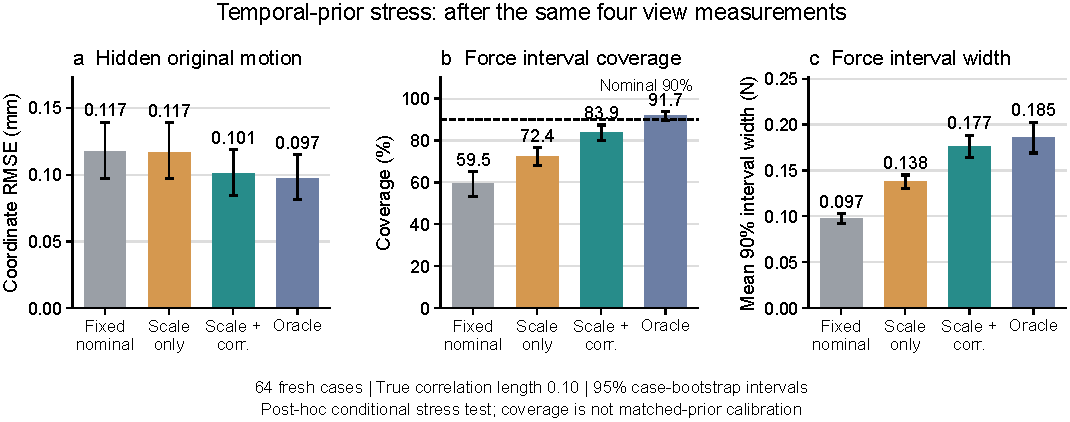
\includegraphics[width=.98\textwidth]{figures/temporal-comparison.pdf}
\caption{\textbf{Temporal uncertainty partially repairs a recognized failure.} Fresh 64-case conditional stress test after four fixed views. Error, coverage and width are shown together, with stratified case-bootstrap 95\% intervals. The covariance oracle is given true amplitude scale and correlation length, not true material or force history.}
\end{figure*}
